Computers have been employed to solve complex computations that would be tedious and time consuming for a human to conduct. These typically deal with executing well-defined sequences of instructions on data, very rapidly. However, computers can only be used as problem-solving tools if both, the problem is well specified, and its solution is tractable. Computers are typically designed to allow the evaluation of a complex sequence of mathematical operations rapidly; this gives them their apparent problem-solving ability. However, to obtain a solution, a computer must first be supplied with a set of instructions or an algorithm, the construction of which is only possible if the steps to the solution can be formalized in codified. 

The prediction of the landing spot of a projectile is an example of such a problem. The rules concerning the descent of the body are governed by the laws of physics which may be precisely specified to a computing system, thus leading to the calculation of the correct answer. On the other hand, if the solution to the problem is not deterministic, it may not be possible to arrive at an answer. Pattern/outliers recognition, trend prediction are examples of such kinds of problems. Many real-world problems are traditionally solved numerically based on certain approximation models. If the model is not known beforehand, it is not possible to compute an answer. The model is also inflexible to change in input trends. Machine learning based approaches attempt to discover trends in the data and thus construct a data-driven model, make predictions or adjust the internal parameters of the model depending on changing trends in the data to better it's performance or improve prediction.

\section{Learning Machines}
A learning machine is one that has the ability to adjust its internal workings (code, data or model) to allow it to gain efficiency or accuracy in its task in response to external information or feedback~\cite{mohri2012foundations}. It is a machine that can learn from its errors and minimize them on future input samples. A learning machine in a lot of ways functions exactly the way human beings animals learn about the world around them. We tend to learn from the statistical dependencies of our actions to the consequences. Over time we adapt our behavior to maximize the rewards from the circumstances. Often the judgment of this reward and consequence itself is based on several factors. The human brain has the ability to generalize previous experiences and apply them to the current circumstance to come up with an optimum decision. Learning machines attempt to mimic this soft computing ability in order to come up with solutions.

It is reasonable to question as to why a machine must be designed to learn; why can it not be constructed such that it performs its task optimally in the first place. It is not always possible to design a machine that can anticipate all variables and variations in input, environment or its own internal workings. Despite the best efforts of human designers, it may not be able to completely characterize the system. Thus, a machine that adapts on the fly will be more suited to handling situations not envisioned initially. The input data volume might be so large that it would take a long time for humans to codify it completely. A machine that gradually learns patterns from the data, in this situation would be able to capture far more information from the data.

The data itself may be subject to a trend, that is there may be a co-related change in some aspects of the data which are consequences of some external influencing factors. Machines that adapt to changes in inputs need not be resigned to accommodate that. Google designed a system that co-related Internet search terms with the spread of flu, allowing them to make predictions about the spread of winter flu in the United States~\cite{ginsberg2008detecting}. However, the system failed to adapt to the change in Internet search behavior during the pH1N1 epidemic in 2009, which caused the system to produce incorrect results~\cite{10.1371/journal.pone.0023610}. In such cases, machines that can learn from and adapt to change in data trends will exhibit superior performance. 


%	\begin{figure}
%	\centering
%	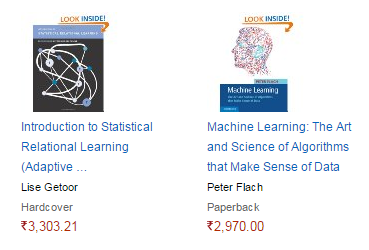
\includegraphics[width=0.4\textwidth]{Figures/amazon_reco}
%	\caption[Screen-shot of the Amazon book recommendation system.]{Books recommended by amazon.in while viewing the book "Predicting Structured Data" by Gokhan Bakir. It is desirable for the vendor to advertise related products in it's catalog.}
%	\label{fig:amazon}
%	\end{figure}


Learning algorithms have been applied to solve a variety of problems including, text or document classification, e.g. spam detection, subject identification, natural language processing, e.g. speech to text, part of speech tagging, computer vision, e.g. image classification, object identification, unassisted vehicle control, e.g. robot navigation, driver aids, optical character recognition (OCR), fraud detection (credit cards, telephones), network security e.g. intrusion detection, denial of service attack prevention, computational biology, e.g. protein function prediction medical diagnosis, recommender systems, e.g. search engines, related content identification, clustering systems, e.g. news collation, related tag identification;




This list is by no means exhaustive, and every day, learning algorithms are being used in new applications every day. It is possible to identify a number of broad templates to address like natured problems. Typical tasks for learning machines can be identified as,~\cite[7-10]{smolaML}
\begin{itemize}
\item \textbf{Binary Classification} involves the separation of input data into two classes. For instance, the example shown in Figure~\ref{fig:binclass}. In other words, given a pattern $x$ drawn from a domain $\chi$, the task is to estimate the value of an associated binary random variable $y \in {\pm1}$. The final decision may be depended on the input pattern, or on the sequence of input patterns. 

	\begin{figure}
	\centering
	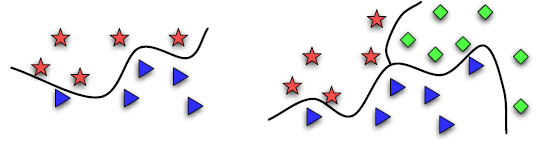
\includegraphics[width=0.7\textwidth]{Figures/classification}
	\caption[Illustration of classification.]{Binary classification (left); separate the stars from triangles. In this example it is possible to do so by drawing a straight line. This serves as an example of a \emph{linear classifier}. Multiclass Classification (right): 3-class classification is shown. Note that in the
	latter case we have a greater degree for ambiguity. For instance, being able to
	distinguish stars from diamonds may not suffice to identify either of them correctly,
	since we also need to distinguish both of them from triangles.}
	\label{fig:binclass}
	\end{figure}	

\item \textbf{Multi-Class Classification} is an extension of the binary classification problem, where the set of lables may assume a larger set of values, i.e. $y \in {1,\ldots,n}$. For instance we may want to classify emails into categories (Work, Personal, Promotions, Subscriptions, \ldots) according to the contents and the sender's address.  See Figure~\ref{fig:binclass} for an example. 
\item \textbf{Structuted Estimation} is an evolution of the multi-class classification problem. It attempts to improve the multi-classification results based on a known structure. For example an ontology may be used while attempting to classify research papers or seasonal temperature information may be used to aid iceberg detection.
\item \textbf{Regression} aims to estimate a real-valued variable $y\in\mathbb{R}$ given an input pattern $x$ (see Figure~\ref{fig:regs}). For instance, we might want to estimate the adrenaline level in a patient based on a blood cortisol measurement.

	\begin{figure}
	\centering
	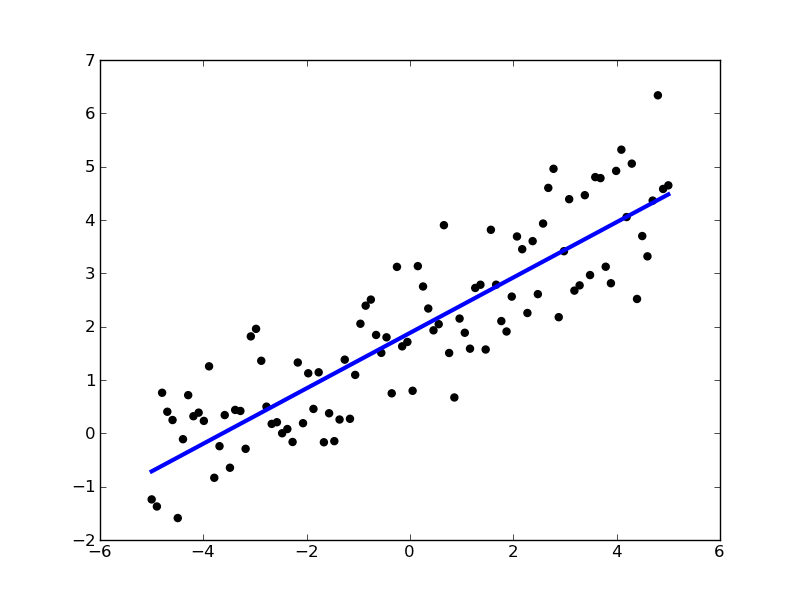
\includegraphics[width=0.5\textwidth]{Figures/regression}
	\caption[Illustration of regression.]{We are given a number of instances (indicated by the dots) and would like to find some function $f$ mapping the observations such that $f(x)$ is close to the input values.}
	\label{fig:regs}
	\end{figure}

\item \textbf{Ranking} is the task of using related parameters to order a set according to some predefined criterion. Internet search rankings are a common example of such a problem where we must rank and sort web pages according to their relevance to the search terms. 
\item \textbf{Clustering} involves the partitioning of input patters into homogeneous groups. For instance, using social media data to group people according to their interests.
\item \textbf{Dimensionality reduction or Manifold learning} involves the transformation of a representation of data into a lower dimensional representation with minimal loss of information. Hyper-spectral images have very high dimensionality (several hundred bands) which can be difficult to work with for computer vision tasks. By discarding irrelevant and redundant information, the dimensionality can be lowered.  
\end{itemize}

\section{The Problem of Representation}

	\begin{figure}
	\centering
	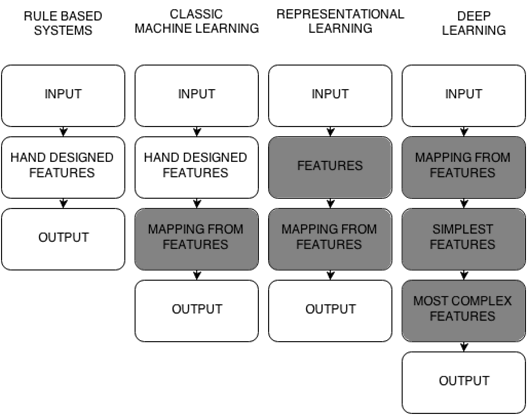
\includegraphics[width=0.7\textwidth]{Figures/deeplearning}
	\caption[Evolution of machine learning.]{Rule based systems are constructed to follow certain hand designed features and generalize poorly when unseen examples are presented. Classical machine learning attempts to learn a mapping from hand designed features, this gives it its generalization ability, however the task of designing the features itself is tedious. Representational learning aims to learn the features from the presented data, however this problem can become as difficult as the original problem itself. The shaded boxes represent the components that are able to learn from data. }
	\label{fig:deep}
	\end{figure}
	
Input data to a machine learning system can be represented in many ways, but some representations help improve the ability of a machine learning algorithm to extract knowledge from the supplied data. For example, numbers represented in the familiar binary notation may not always be successful in machine learning applications, and a one-hot representation may be preferred. The one hot notation involves setting successive bits high for successive numbers. For example, 1 is represented as $“0001”$, 2 as $“0010”$, 3 as $“0100”$ and so on. In a traditional binary representation, numbers that are in proximity to one another have very little similarity, for example 7 $(0000 0111)$ and 8 $(0000 1000)$ are separated by just one position on the number line, yet have no bits in common, while 64 $(0100 0000)$ and 1 $(0000 0001)$, which are quite far apart are separated by just one bit in the representation. This causes the learning machine to generalize poorly and will affect the performance of the architecture~\cite{Bengio-et-al-2014-Book}.

A lot of applications of machine learning involve input data that cannot be directly represented numerically. Computer vision for instance deals with images, the classification of spam email deals with raw text written in human languages. It becomes important to convert this input to a system that can be numerically encoded for input to the learning machine. The chosen parameters, which are used to represent a certain property of the data, are called features. The operation thus is a transformation of the data into the feature space. For instance, in an image corner points, lines and edges may be considered to be featured. In voice recognition, the pitch of the audio sample can be considered to be a feature.

Representation of the data is thus a central problem in the design of any machine learning algorithm. For many real-world applications, the selection of an appropriate representation scheme can be dauntingly difficult. One solution is to use a machine learning technique itself to capture not just the mapping from input to output but also the representation. This technique is called \emph{representational learning}~\cite{bengio2013representation}.

Learned features can offer a higher performance, and save human time and effort that would have been spent in constructing a hand designed model. However, identification of the features is not a trivial task.
\emph{Factors of variation} are used to examine the relation between the input data and the data. These factors may not be directly present or sensed in the data, but rather exist in the human mind that allows us to discriminate and make inferences about the data. These may be concepts and abstractions that help us process and understand the data.  


In the real world, every data sample is affected by a wide variety of factors, and it becomes important to separate these factors from the data, for instance, a tennis ball may become discolored over the course of a match, and the shape of the ball itself changes on impact. In this situation obtaining a representation of the data requires a human-like understanding of the data. In this situation, representational learning may not be helpful because the complexity of obtaining the representation is comparable to the solution of the original problem in itself.

	\begin{figure}
	\centering
	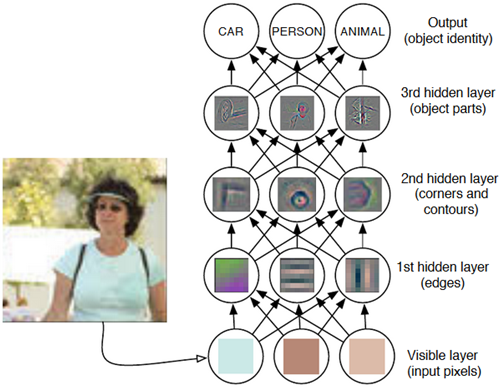
\includegraphics[width=0.6\textwidth]{Figures/deeplearning2}
	\caption[Illustration of deep algorithms.]{Deep learning algorithms attempt to represent the problem as a series of simpler sub-tasks. In the example shown, the task of recognizing the object in the image, is broken down into tasks of recognizing the edges in the image, then the corners in the next layer, then finally object parts in the third layer, which eventually leads to the identification of the object.  Image courtesy Zeiler and Fergus, Springer~\cite{zeiler2014visualizing}.  }
	\label{fig:deepimg}
	\end{figure}

\section{Deep Learning}

	\begin{figure}
	\centering
	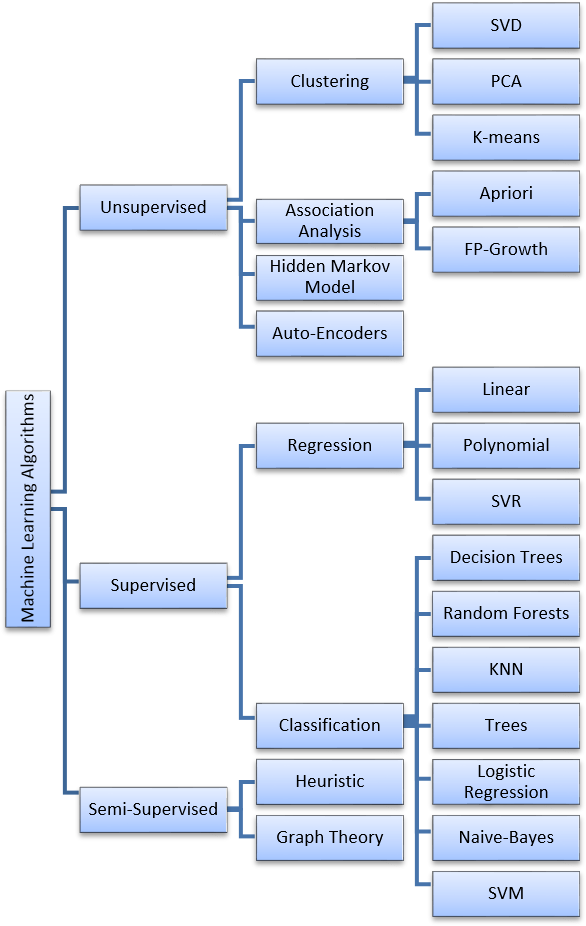
\includegraphics[width=0.7\textwidth]{Figures/MLtypes}
	\caption{Broad classification of machine learning algorithms by the nature of their training.}
	\label{fig:mltypes}
	\end{figure}

It can be difficult to learn high-level features from data. Deep Learning attempts to solve this by representing the original problem in a series of simpler sub-representations. The depth of the architecture refers to the number of levels of a composition of non-linear operations in the function learned. It allows the learning algorithm to learn a complex abstract concept from a series of more straightforward concepts. The multiple levels of abstraction will enable a system to learn complex functions mapping the input to the output directly from data, without depending on features crafted explicitly. At each level, features can be added to the representation. Thus it is not necessary to deal with all the features at once, like in shallow learning, allowing a more efficient way of dealing with a more complex representation. Deep learning breaks down the learning of the features into a pipeline where first simpler features are learned, which lead to the processing of increasingly complex features. 



In Figure~\ref{fig:deepimg} the task of object recognition is represented with a deep learning approach. At the first layer, we have the input pixels. This visual information is immediately recognizable to the human vision system, but is of little use to a leaning machine and is too complicated to map the object identity from a set of pixels. Learning at this stage is nearly impossible. We now break this complicated task into simpler sub-tasks, each dealing with a different layer of the representation. 
\begin{itemize*}
\item The first layer of the learning machine looks for the edges in the image by comparing pixel values of individual pixels with that of their neighbors. 
\item Once the edges have been represented, the next layer can represent the contours and corners as a set of edges. 
\item This, in turn, allows the third layer to group together these features to begin to identify object parts. 
\item Finally the output later can relate the parts to identify the object.
\end{itemize*}  

%\section{Recent advances in remote sensing}
%Despite the availability of 


\section{Classification of Remotely Sensed Images}
Classification of remote sensing images involves the grouping of pixels a scene or dataset into homogeneous groups, usually representing land cover classes or "themes". This categorized data can then be used to produce thematic maps of the areas represented in the image. Generally this is used to map distinct land-covers types like agriculture, urban and built up, forested, desert areas etc. The selection of the covers classes are application dependent, however certain standardized classification systems like the National Land Cover Data (NLCD) have been used operationally. The NLCD is a 21-class land cover classification scheme applied developed by the USGS Land Cover Institute for use in conjunction with Landsat Thematic Mapper data~\cite{jin2013comprehensive}. 

Usually multi-spectral data, like that from the Landsat mission, is used to perform classification.  The spectral pattern present for each pixel is used to discriminate the classes~\cite{lillesand1979remote}. These datasets allow for fairly accurate classification of large areas of the Earth's surface.  Data from the advanced very-high-resolution radiometer sensor (AVRIS) sensor aboard National Oceanic and Atmospheric Administration's (NOAA)  operational series of meteorological satellites was used by~\cite{Tucker25011985} to classify land-cover types and monitor changes in vegetation over the continent of Africa. At larger scales,~\cite{de1998global} generated a global land-cover classification dataset at a spatial resolution of 8-km using space-borne multi-spectral imagining systems and a decision tree classifier. A higher resolution dataset was derived from the Moderate Resolution Imaging Spectroradiometer (MODIS) sensor on-board Terra by~\cite{friedl2002global}. They generated a global land-cover map with a spatial resolution of 1-Km and using primarily the International Geo-sphere-Biosphere Programme Data and Information System (IGBP-DIS) classification scheme~\cite{Loveland97IGBP}.

Data from several medium resolution multi-spectral sensors like AVRIS, MODIS and Landsat TM have been used successfully for such applications due to their continuous global coverage, data availability and high spectral information content. However these sensors do have certain restrictions. They can not image during the night as they are dependent on the incident solar radiation for imaging. Cloud cover can also affect the quality of images as these sensors are unable to image though clouds. This is especially more of a problem while imaging areas covered with snow, as it can become difficult to differentiate the white snow covered land area from the white clouds. 

To overcome these problems, increasingly Synthetic Aperture Radar (SAR) data is being used for thematic map generation, especially over the cryosphere~\cite{jezek1998radarsat}. Certain applications also places temporal restrictions on the generation of thematic maps. For example, to generate ice-breg warning maps, the data can be acquired in a limited window and rapid and timely updates of these maps becomes critical~\cite{skvarca1994changes}. In such cases, it is also desirable to be able to produce these maps, operationally with a high degree of automation. 

Polarimetric SAR (PolSAR) imaging is an advancement made on single polarization SAR imaging. The polarization of the incident wave is controlled so that it is restricted alternatively to either H or V transmission. Similarly, reception is performed alternativly in H or V polarizations, so that for every imaged pixel, four combinations of polarization i.e. HH, HV, VH and VV are captured. PolSAR imaging can capture more information about the physical properties of the target than possible with single or dual polarization imaging, and consequently, this can lead to better classification~\cite{Lee2001multipolclass}. 

	\begin{figure}[tbp]
	\centering
	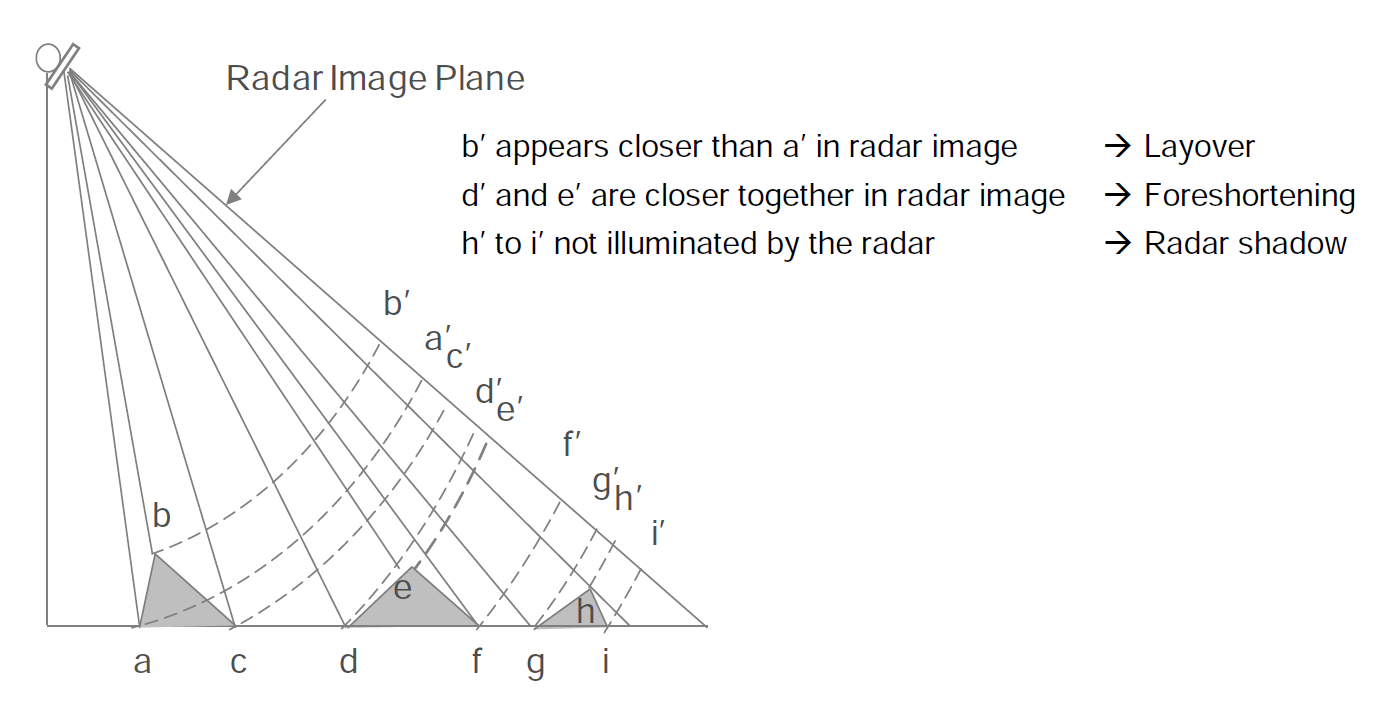
\includegraphics[width=\textwidth]{Figures/geometricSAR}
	\caption{Geometric distortions in SAR imaging due to the side looking geometry.  Image courtesy VanZyl, Wiley~\cite{van2011synthetic}.  }
	\label{fig:sargeo}
	\end{figure}
	

\section{Challenges in SAR Image Classification}

SAR imaging introduces its own set of challenges to the classification problem. Being an active sensor, it must supply the illuminating energy, i.e. radar pulses, which necessitates that a power source be tethered to the sensor. Satellite sensors are usually powered by a battery which is rechargeable by solar energy. This limits the sensors continuous operation capability. Unlike optical sensors, which can be operated continuously, a typical modern spaceborne SAR sensor can only be operated for ~11 minutes per ~90 minute orbit~\cite{simpson2004terrasar}. This makes it difficult to generate the updated global mosaics that are generated using multi-spectral sensors~\cite{stockli2005blue}. Additional, in PolSAR mode, because each pixel is imaged twice on two subsequent pulses, the effective swath width of the imaged strip is half as compared to a single polarization SAR system. This somewhat reduces the feasibility of PolSAR in generating thematic maps of large areas. 

	\begin{figure}[tbp]
	\centering
	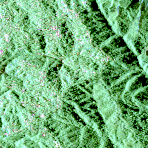
\includegraphics[width=0.4\textwidth]{Figures/shadow}
	\caption{Crop of a Pauli RGB image generated from a UAVSAR dataset showing layover (bright) and shadow (dark) areas.  }
	\label{fig:sarshadow}
	\end{figure}
	


Unlike optical images, which are acquired with the sensor facing towards the nadir, SAR images are acquired in side look geometry~\cite{lee2009polarimetric}. RADAR images are formed by fundamentally from the echoes returned from targets, thus a RADAR that faces vertically down would not be able to distinguish echos from equidistant targets that lie on either side of the sensor. In non imaging radars with a narrow beam-width, like sounders, this behavior is desirable, but it makes imaging impossible. The side looking geometry introduces geometric artifacts like layover, foreshadow and shadow effects. This causes elevations in the imaged terrain (buildings, hills and mountains) to suffer from certain distortions in the produced image~\cite[21]{van2011synthetic} as shown in~\ref{fig:sargeo}. Along with the shape distortion, foreshortening also manifests as an area of bright RADAR return, which can cause the land-cover type in these areas to mis-classified. Similarly, shadow regions appear dark in the image and contain no echo information, making classification difficult as shown in Figure~\ref{fig:sarshadow}

\begin{figure}
\label{fig:statistics}
 \centering
        \begin{subfigure}[b]{0.65\textwidth}
                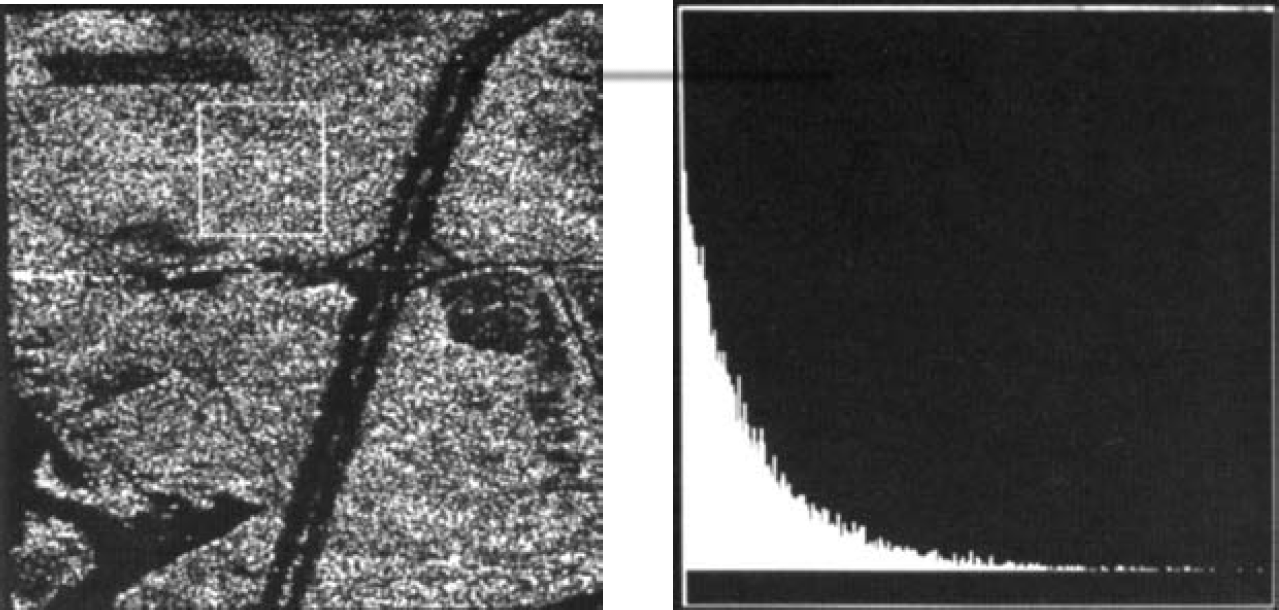
\includegraphics[width=\textwidth]{Figures/lee1}
                \caption{}
                \label{fig:stat1}
        \end{subfigure}%
        \hspace{0.1em}
        \begin{subfigure}[b]{0.65\textwidth}
                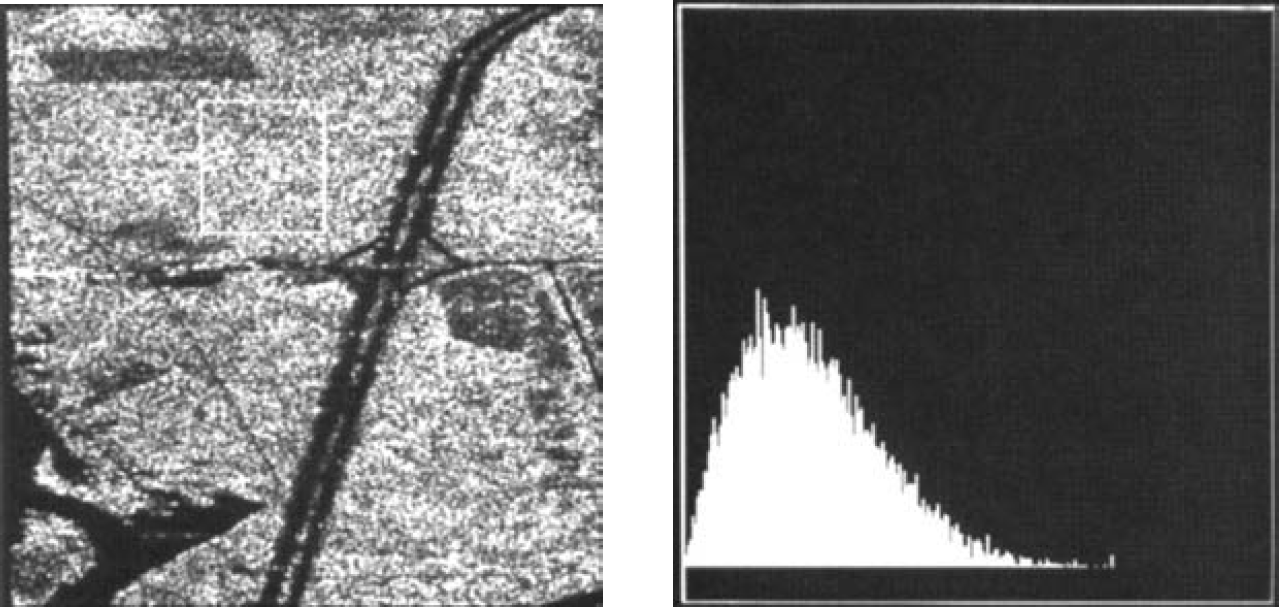
\includegraphics[width=\textwidth]{Figures/lee2}
                \caption{}
                \label{fig:stat2}
        \end{subfigure}%
        \hspace{0.1em}
        \begin{subfigure}[b]{0.65\textwidth}
                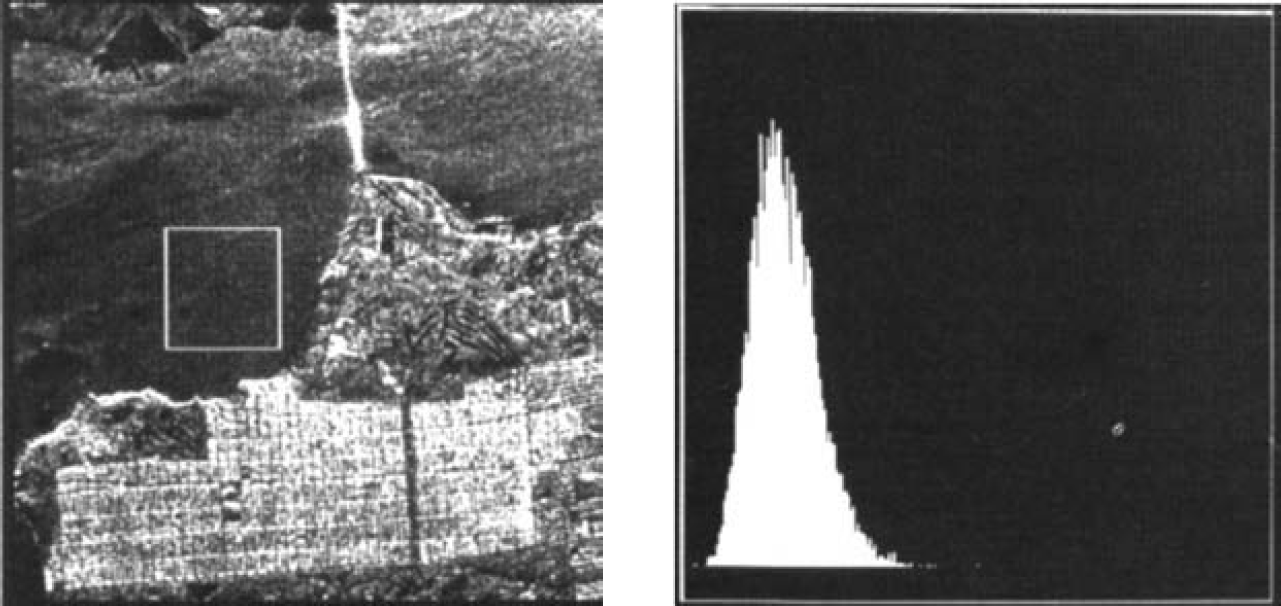
\includegraphics[width=\textwidth]{Figures/lee3}
                \caption{}
                \label{fig:stat3}
        \end{subfigure}%

             
\caption[SAR speckle statistics]{ SAR speckle distribution are plotted for intensity and amplitude images of different looks. (~\ref{fig:stat1})  1 Look intensity SAR image with it's histogram (exponential distribution). (~\ref{fig:stat2})  1 Look amplitude SAR image (same area as before) with it's histogram (Rayleigh distribution)   
(~\ref{fig:stat3})  4 Look amplitude SAR image with it's histogram (chi distribution).
Figure courtesy Lee and Pottier~\cite[104]{lee2009polarimetric} }
\end{figure}

Apart from the problems related to the physical constraints of the images, like other coherent imaging techniques, suffers from the problem of speckle~\cite{gagnon1997speckle}. Speckle noise can complicate the task of classification of SAR images. Further, the speckle pattern is non often non-Gaussian in distribution, thus filtering and classification techniques that have been developed for Gaussian optical images can not be directly applied to SAR images. Various non Gaussian models have been proposed to represent SAR data~\cite{jakeman1976model}. To represent PolSAR data multivariate K distribution based models have been proposed~\cite{lee1994k}, ~\cite{doulgeris2010scale}. This was further extended by~\cite{freitas2005polarimetric} who used the G distribution to model the speckle pattern. Non Gaussian model based classification techniques have been applied by~\cite{akbari2010non} to segregate glacier ice types to track changes in the glacier.  Various statistical parameters which can be exploited in conjecture with machine learning techniques to alleviate some of the challenges of the classification of PolSAR images.

\section{Generative and Discriminative Classifiers}
Generative classifiers learn a model of the joint probability, $p(x|y)$, where $x$ represents the inputs and $y$, the labels. They make their predictions according to the $p(x|y)$ computed using the Bayes rule and then selecting the label $y$ with the highest probability. Discriminative classifiers model the posterior $p(y|x)$ directly or learn from a direct map from inputs $x$ to class labels. It is more attractive to use discriminative classifiers are over generative ones. According to~\cite{vapnik1998statistical}, the classification problem should be solved directly and not as an intermediate step such as modeling of the probability $p(X|y)$. An experimental comparison of this can be found in~\cite{ng2002discriminative}.

